\chapter{FLC100 shield assembly}

\section{Introduction}
The FLC100 shield is an Arduino ``shield'' which operates at
\volt{3.3}. Do not attempt to use it with standard Arduino boards
which are operated at \volt{5}. The shield houses the XRF radio
module, the boost power supply (which creates the \volt{3.3} supply
for the microcontroller and radio) and the \volt{3.3} -- \volt{5} level
shifters.

There are both through-hole and surface mount versions of the boost
power supply. It is suspected that the through-hole version causes
\rfi\ since the radio module often fails to receive messages. This
problem was not apparent on the prototype board. The surface-mount
version has no such problems and is the option which should be
used. It is also cheaper and more efficient.

There is an option to fit a FLC100 sensor directly to the circuit
board. This option is not used because the FLC100 is slightly
temperature sensitive and better performance is obtained by
positioning the sensor below ground. Whilst the board provides an
option to fit an MCP3424 \adc\ and MAX619 charge-pump power supply they
are also fitted remotely, below ground, for reasons of temperature
stability.

\section{FLC100 shield version 1.0}

\begin{figure}
  \centering
  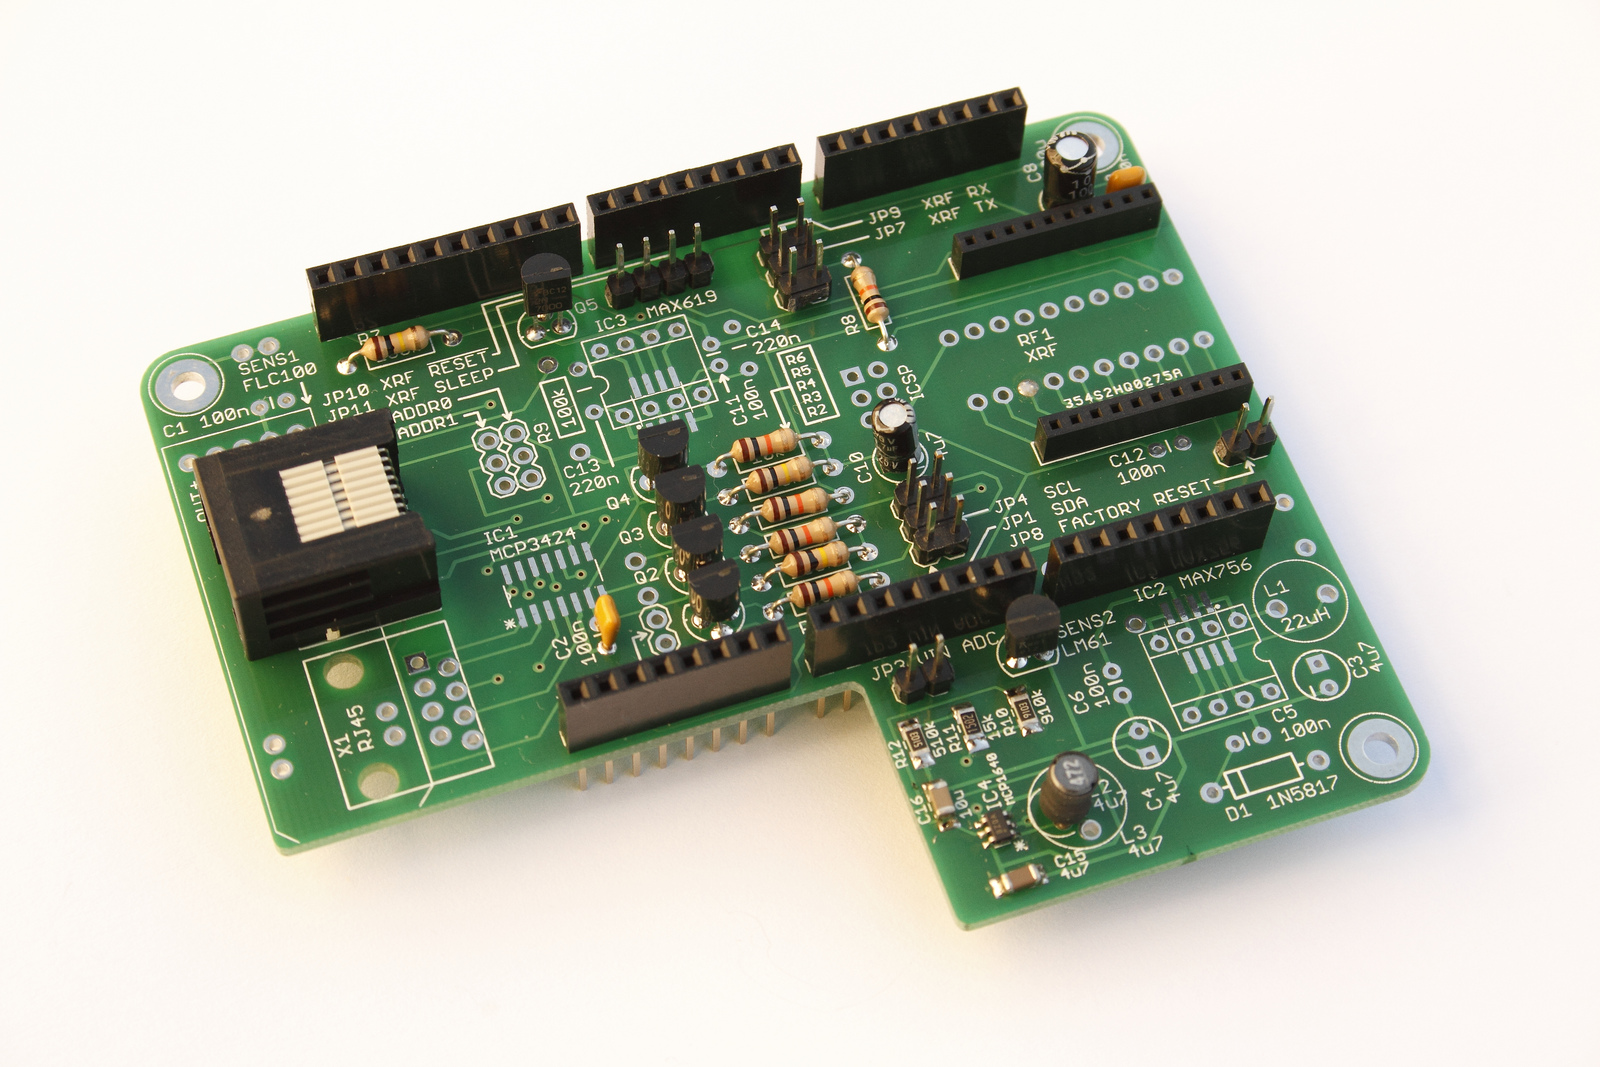
\includegraphics[keepaspectratio,width=\textwidth]{%
    images/flc100-shield}
  \caption[Completed FLC100 shield]{Completed FCL100 shield. %
    \photoCredits{%
      \href{http://www.flickr.com/photos/stevemarple/10787109594/}{%
        \copyright Steve Marple. CC BY-SA 3.0.}}}
  \label{fig:flc100-v1.0}
\end{figure}

\subsection{Order of assembly}
\begin{buildorder}
\item IC4 (MCP1640).
\item R12 (\kohm{510}).
\item R11 (\kohm{15}).
\item R10 (\kohm{910}).
\item C15 (\uF{4.7}).
\item C16 (\uF{10}).
\item R1, R3, R4, R6, R8 (\kohm{10}).
\item R2, R5, R7 (\kohm{100}).
\item C2, C7, C9 (\nF{100}). \todo[check list]
\item C10 (\uF{4.7}).
\item C8 (\uF{100}).
\item L2 (\uH{4.7}). The shorter lead should be fitted
  \todo[\ldots]. Although the orientation of inductors is normally
  ignored communication with the manufacturer revealed that the
  shorter lead indicates the start of the winding. This arrangement is
  preferred to help minimise \rfi.
\item
\item
\item
\item
\item
\item Q1, Q2, Q3, Q4, Q5 (2N7000).
\end{buildorder}

\begin{landscape}
  \begin{figure}[p]
    \centering
    \includegraphics[keepaspectratio,width=28cm,height=16cm]{%
      images/FLC100_shield_v1_0_sch}
    \caption{FLC100 shield v.~1.0 circuit diagram.}
    \label{fig:flc100-shield-v1.0-cct-diag}
  \end{figure}
\end{landscape}

